\section{Bargaining over a rival's opportunity}
\label{sec:bargaining}

\subsection{The completion contrast depends on the offer}
The agents negotiate selectively. Across 526 threads, 920 responses comprise 113 acceptances, 394 counters and 413 rejections. Acceptance is legal in 918 cases. Sol and Opus counter most often, whereas Gemini and Grok reject most often; each nevertheless accepts between 26 and 30 offers (Table~\ref{tab:responses}). A common settlement count conceals different ways of disagreeing.

\begin{table}[t]\centering\small
\begin{tabular}{@{}lrrrr@{}}\toprule
Recipient & Responses & Accept & Counter & Reject\\\midrule
Sol&235&30&140&65\\
Gemini&242&26&36&180\\
Opus&189&29&141&19\\
Grok&254&28&77&149\\\bottomrule
\end{tabular}
\caption{All negotiation responses. Opus uses action-only recovery in 162 of its 189 responses. Grok's call disagrees with assistant content in seven acceptances, one counter and three rejections.}
\label{tab:responses}\end{table}

We first compare offers asking the holder to part with a deed. Among opening offers, author-only completion requests receive 138/187 rejections (73.8\%), compared with 105/176 (59.7\%) requests completing neither party. This pooled contrast combines different exchanges. A swap transfers deeds in both directions and can include cash; a pure cash bid offers cash for deeds, without a reciprocal deed or jail card.

Separating those forms changes the result (Table~\ref{tab:opening}). Opening swaps completing only the proposer receive 95/116 rejections (81.9\%), compared with 37/72 (51.4\%) for swaps completing neither party. Pure cash bids show no corresponding increase: 42/70 (60.0\%) versus 67/103 (65.0\%). The record therefore supports a form-dependent completion contrast, not a general reluctance to sell every completing deed. Both positions and counterparties differ across these offers; the contrast is observational.

The opening swap ordering holds in all five seed blocks and for every recipient configuration. It also survives excluding threads opened by Grok calls that conflict with assistant content: 93/112 versus 26/43. That exclusion leaves the direction positive in four of five seed blocks. In later swaps, rejection is 8/39 versus 7/34; later cash bids receive 13/61 versus 13/73. Later offers are selected by what both parties have already accepted or resisted. Neither the smaller later differences nor the opening contrast identifies an effect of negotiation or offer form.

\begin{table}[t]\centering\small
\begin{tabularx}{\linewidth}{@{}lYrrrr@{}}\toprule
Opening form & Completes & Offers & Accept & Counter & Reject\\\midrule
Swap & Proposer only & 116 & 1 & 20 & 95 \\
Swap & Neither & 72 & 17 & 18 & 37 \\
Cash bid & Proposer only & 70 & 2 & 26 & 42 \\
Cash bid & Neither & 103 & 4 & 32 & 67 \\
\bottomrule\end{tabularx}
\caption{Opening responses by offer form. Swaps exchange deeds in both directions and may include cash. Pure cash bids offer cash for deeds without reciprocal deeds or jail cards. Completion is evaluated after the proposed transfer. The two other opening deed requests in these completion categories are both rejected; the full 918-offer table is in the appendix.}
\label{tab:opening}\end{table}


The agents' stated reasons connect that pattern to economic consequences. Two LLM-assisted readings agree that 61 of 74 rejections of offers completing the recipient's own group name a trade-linked consequence for the rival. This includes 27/38 recipient-only completions and 34/36 offers completing both parties. Gemini and Grok contribute 56 of the agreed cases, and G1 and G15 contribute 31. The concentration matters: these statements support the presence and content of strategic attention, rather than a validated population rate of correct reasoning.

\TranscriptTitle{g15}{Refusing one's own monopoly to withhold the rival's}
At G15 turn 63, Sol has \$730 and Grok \$333. Sol offers two greens for Ventnor and \$100, completing both groups. Grok's note compares what the two players could then build:
\TranscriptQuote{fx-g15-refusal-note}
Sol removes its cash request, adds Kentucky, and finally offers the two greens, Kentucky and \$250. Grok still refuses:
\TranscriptQuote{fx-g15-final-refusal}
The first offer's post-trade cash figures, \$830 and \$233, are correct. A full first layer on green costs \$600, although one legal house costs \$200. Grok is considering the rival's immediate development opportunity, not merely whether it receives a monopoly. All three offers fail. Eighteen turns later its blockers pass to Gemini through bankruptcy, and Sol never completes either group. That continuation does not establish whether accepting would have been better.
\TranscriptSource{G15 d168--175, standard responses. Quoted public messages occur in the next counterparty requests.}

\subsection{Prices, counters and concessions}
A refusal does not exhaust the bargaining response. Of 111 counters to author-only completion offers, 79 keep the entire noncash exchange while improving the counterer's cash. The same happens in 81 of 110 counters to non-completing deed requests. Cash repricing is thus common across the comparison populations; it is not uniquely a charge for completing a rival's group.

Unchanged-bundle concessions provide another view. In 58 offers, an author improves the other party's cash without changing the noncash bundle, while the exchange would complete only the author's group. Nine are accepted. Among 56 such concessions that request a deed but complete neither party, 17 are accepted. These are repeated, selected negotiations, not interventions on price. They show that adding cash often leaves the disagreement unresolved.

For single-deed cash asks, the median price relative to board purchase price is higher for a completing buyer within each of six Sol/Opus/Grok-by-mortgage-status cells. This is context-sensitive asking, but the size and origin of a completion premium remain unresolved. Of seven same-game, same-seller, same-deed comparisons, six retain the same mortgage status: completing-buyer asks are higher in four, lower in one and equal in one, whether using medians or first asks. G4 compares the deed before and after mortgage and changes direction with the summary chosen. Time, buyer and negotiation history still differ within the six same-status comparisons (Appendix~\ref{app:comparisons}). Buyer bids likewise vary by system rather than showing a common premium.

\begin{figure}[t]\centering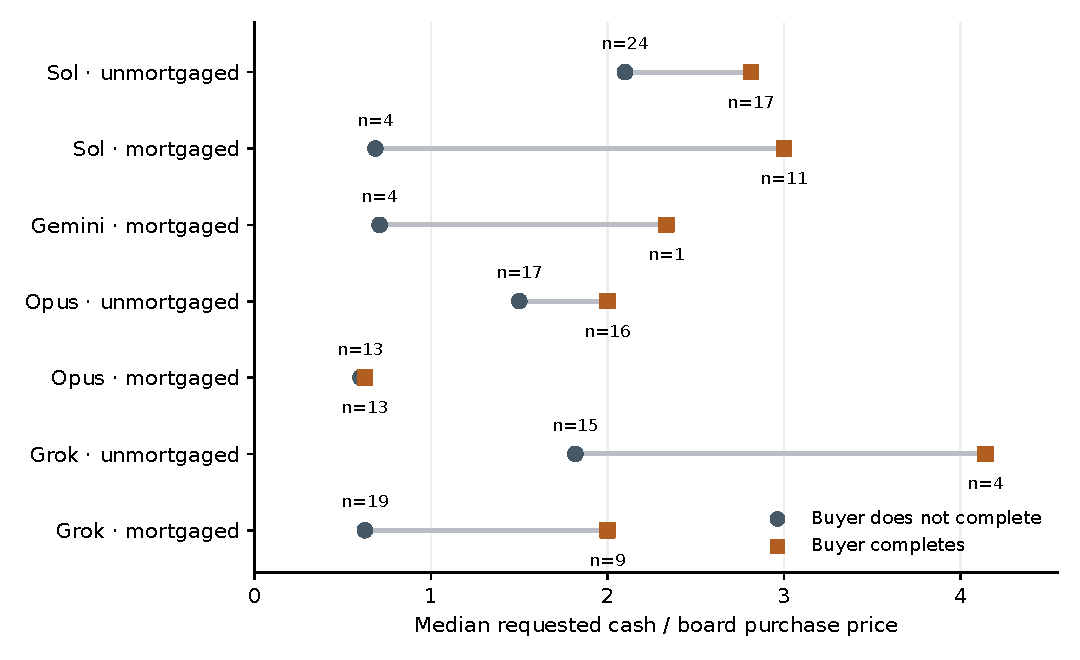
\includegraphics[width=\linewidth]{asking_prices.pdf}
\caption{Median single-deed asking prices divided by board purchase price. Labels show offer counts. Each row holds seller and mortgage status fixed; deed, buyer, time and negotiation history can differ. The pattern concerns asks, not a price premium identified from matched transactions.}
\label{fig:prices}\end{figure}

\TranscriptTitle{g2}{Pricing the buyer's next move}
At G2 turn 45, Opus holds two yellows and bids \$325 for Sol's Marvin Gardens. Sol responds:
\TranscriptQuote{g2-d124-price}
One turn earlier Sol asked Grok, which owned no yellow, for \$450 for the same deed. Its note now discusses Opus's remaining construction cash. The stated \$520 remainder is correct, but its claim that this buys nine yellow houses is not: houses cost \$150 each. Opus publicly calls \$450 final while retaining a private \$475 contingency. Sol refuses:
\TranscriptQuote{g2-d128-keep}
At turn 69 the roles reverse. Opus has \$17 and sells its two yellows to Sol for two railroads plus \$100. Sol builds, later sells those buildings, earns \$44 undeveloped yellow rent and no developed yellow rent, and eventually loses the group to Gemini through bankruptcy. The sequence connects the expressed concern about what the buyer can build to a later reversal of who can finance the group. Different asks and a concrete rationale are observed; neither establishes the best price.
\TranscriptSource{G2 d119--128 and d197--198; undeveloped rent at event 1566. Opus's initial bluff is a standard response, its later sale uses recovery.}

\subsection{Evaluating the bargain separately from the pitch}
A recipient can accept terms while rejecting the explanation used to sell them. This distinction is central when language and structured action disagree.

\TranscriptTitle{g19}{Correcting a false premise without rejecting the trade}
Grok's received proposal offers Virginia and \$150 for States, claiming:
\TranscriptQuote{g19_d135_false_public}
Both properties are pink. The same response's private note says to abort the trade, and assistant content names an end action. The received proposal nevertheless reaches Sol, which replies:
\TranscriptQuote{g19_d136_correction_accept}
The exchange executes and completes no group. Sol's note judges the terms favorable. This is a positive example of separating a factual premise from the transaction's terms. It is not evidence that the pitch persuaded Sol, and Grok's incompatible channels do not support treating the false statement as a coherent intention across its entire response.
\TranscriptSource{G19 d135--136, standard attempts; Sol's stored request contains the false message.}
